\section{Theory uncertainties in a limit}\label{sec:21.4}

A silicon detector that records no event above a one-pair threshold in a kilogram-year excludes, at \SI{3}{MeV} and for a heavy mediator, every cross-section above $\SI{1.24e-41}{cm^2}$, if the rate is the central value of \cref{we:10-band3}. With the rate computed at the random-phase level, without local fields, the same zero excludes everything above $\SI{9.23e-42}{cm^2}$, a limit 1.35 times stronger. The central rate is itself uncertain by a factor of 1.48 at one standard deviation. Which number should the experiment publish, and how wide is the uncertainty on it?

\subsection{Poisson limits with a known background}\label{sec:21.4-poisson}

A counting experiment observes $N_{\mathrm{obs}}$ events where its background is expected to give $N_{\mathrm{bkg}}$. The classical upper limit at confidence level $\mathrm{CL}$ is the signal $N^{\mathrm{up}}$ at which data as low as those observed occur with probability $1 - \mathrm{CL}$,
\begin{equation}
  \sum_{n=0}^{N_{\mathrm{obs}}}P\bigl(n\,\big|\,N^{\mathrm{up}} + N_{\mathrm{bkg}}\bigr) = 1 - \mathrm{CL} ,
  \label{eq:21.4-classical}
\end{equation}
with $P$ the Poisson probability \cref{eq:1.5-poisson}, as in \cref{sec:1.5-limit}. For no events the sum has one term, and $N^{\mathrm{up}} = \ln[1/(1 - \mathrm{CL})] - N_{\mathrm{bkg}}$, which is $2.303 - N_{\mathrm{bkg}}$ at \SI{90}{\percent}. The background lowers the limit even though nothing was seen: with $N_{\mathrm{bkg}} = 1$ the limit is 1.303, and for $N_{\mathrm{bkg}} > 2.303$ the interval is empty. An empty interval is a correct frequentist statement, since no events on a background above 2.303 occur in fewer than \SI{10}{\percent} of experiments, but it says nothing about the signal. With one event on a background of one the classical limit is 2.890, and with two on a background of two it is 3.322.

Feldman and Cousins removed the empty intervals by changing the order in which outcomes enter the construction~\cite[Sect.~IV\,A]{feldman1998unified}. At each trial signal $N_{\mathrm{sig}}$ they rank the outcomes $n$ by the likelihood ratio
\begin{equation}
  \mathsf{R}_{\mathrm{FC}}(n) = \frac{P(n\,|\,N_{\mathrm{sig}} + N_{\mathrm{bkg}})}{P\bigl(n\,|\,\max(0, n - N_{\mathrm{bkg}}) + N_{\mathrm{bkg}}\bigr)} ,
  \label{eq:21.4-fc}
\end{equation}
the probability of $n$ at the trial signal over its probability at the best signal that is not negative~\cite[Eq.~(4.1)]{feldman1998unified}. Outcomes are accepted in decreasing order of $\mathsf{R}_{\mathrm{FC}}$ until their summed probability reaches $\mathrm{CL}$, and the interval for $N_{\mathrm{obs}}$ is the set of trial signals whose accepted outcomes contain it. The interval is never empty, and it turns from an upper limit into a two-sided interval as $N_{\mathrm{obs}}$ grows without the experimenter choosing when. Its \SI{90}{\percent} upper ends are 2.44 for no events and no background, 1.61 and 1.08 for no events on a background of one and of three, and 3.36 for one event on a background of one~\cite[Table~IV]{feldman1998unified}. Without background the classical limit is the smaller of the two, since the ordered construction reserves some probability for two-sided intervals that an upper limit does not need. The book quotes classical upper limits, the $N_{90}$ of \cref{sec:1.5}.

The classical and the Feldman--Cousins limit both become a cross-section limit through \cref{eq:1.5-limit}, with $N^{\mathrm{up}}$ in place of $N_{90}$. A search with several bins could quote the smallest of its per-bin limits, but the joint confidence of the smallest per-bin limit is lower than the confidence of each bin unless the confidence levels are corrected by the union bound of \cref{sec:21.2-program}. A likelihood uses all bins at once, and the theory uncertainties enter through it.

\subsection{Theory and detector nuisance parameters}\label{sec:21.4-like}

A search records counts $N_{\mathrm{obs},j}$ in bins $j$ of the measured quantity, pair number for a charge detector, phonon energy for a calorimeter. Its expected signal in bin $j$ is $N_{\mathrm{sig},j} = \sigmae\,M_{\mathrm{det}}t_{\mathrm{exp}}\,r_j(\mchi;\vartheta)$, with $r_j$ the rate per unit cross-section into the bin, computed from \cref{eq:8.7-handoff} with the response $S(\vartheta)$ of \cref{eq:8.8-M} in place of $S$ and one parameter $\vartheta_k$ for each theory uncertainty of the response (\cref{sec:8.8}). The rate $r_j$ generalizes the $r(\mchi)$ of \cref{sec:1.5} to one bin and to nonzero $\vartheta$. With a known background $N_{\mathrm{bkg},j}$, the Poisson probabilities of \cref{eq:1.5-poisson} and a standard normal constraint on each $\vartheta_k$, the likelihood of one exposure is
\begin{equation}
  \mathsf{L}(\sigmae,\vartheta) = \prod_j P\bigl(N_{\mathrm{obs},j}\,\big|\,N_{\mathrm{sig},j}(\sigmae,\vartheta) + N_{\mathrm{bkg},j}\bigr)\;\prod_k\ee^{-\vartheta_k^2/2} .
  \label{eq:8.8-like}
\end{equation}
In statistics each $\vartheta_k$ is a \emph{nuisance parameter}: it changes the expected counts but is not the quantity being measured. The nuisance parameters are removed by profiling~\cite[Eq.~(7)]{cowan2011asymptotic}, \cref{eq:C.14-profile} of \cref{app:C.14}: at each $\sigmae$ every $\vartheta_k$ takes the value that maximizes $\mathsf{L}$. To first order in $\vartheta$, a normalization uncertainty $(1 + \delta_k)^{\vartheta_k} \simeq 1 + \vartheta_k\ln(1 + \delta_k)$ is the Gaussian offset of \cref{app:C.14} with the width $\sigma_\vartheta = \ln(1 + \delta_k)$, and the widths add in quadrature as in \cref{eq:C.14-quadrature}.

One bin with no events and no background shows how much a theory uncertainty costs a limit. With $N(\vartheta) = N_{\mathrm{nom}}(1 + \delta)^\vartheta$, \cref{eq:8.8-like} gives $-2\ln\mathsf{L} = 2N(\vartheta) + \vartheta^2$ up to a constant. The best fit, at $N_{\mathrm{nom}} = 0$ and $\vartheta = 0$, has the value zero. At fixed $N_{\mathrm{nom}}$ the profile condition $2kN(\hat{\hat\vartheta}) + 2\hat{\hat\vartheta} = 0$, with $k = \ln(1 + \delta)$, gives $\hat{\hat\vartheta} = -kN(\hat{\hat\vartheta})$. The nuisance parameter is pulled toward less signal, since no events were seen, and the profiled statistic is $\mathsf{t}_{\mathrm{p}} = 2u + k^2u^2$, with $u = N(\hat{\hat\vartheta})$. The asymptotic thresholds of \cref{app:C.14} fail at zero counts, and for this illustration we set the threshold to the value $\mathsf{t}^* = 2N_{90} = 4.61$ at which the statistic without nuisance parameter reproduces the exact limit $N_{90} = 2.303$ of \cref{eq:1.5-N90}. Solving $\mathsf{t}_{\mathrm{p}} = \mathsf{t}^*$ for $u$ and using $N_{\mathrm{nom}} = u\,\ee^{k^2u}$ gives the factor by which the limit grows,
\begin{equation}
  \frac{N_{\mathrm{nom}}^{\mathrm{lim}}}{N_{90}} = \frac{2w\,\ee^{w}}{k^2\mathsf{t}^*} = 1 + \frac{k^2\mathsf{t}^*}{4} + O(k^6) , \qquad w = \bigl(1 + k^2\mathsf{t}^*\bigr)^{1/2} - 1 .
  \label{eq:8.8-cost}
\end{equation}
The cost is of second order in the size of the truncation: \SI{1.0}{\percent} for $\delta = 0.1$, \SI{8}{\percent} for $\delta = 0.3$ and \SI{19}{\percent} for $\delta = 0.5$. Quoting instead the worst case within one standard deviation, $\vartheta = -1$, costs $1 + \delta$, of first order: \SI{10}{\percent}, \SI{30}{\percent} and \SI{50}{\percent}. The profiled limit and the worst case are different statements, a likelihood and an envelope, and a result must say which it reports. The power form of \cref{eq:8.8-M} matters here as well. A linear form $1 + \vartheta\delta$ can switch the signal off entirely at $\vartheta = -1/\delta$, at the cost of a term $\vartheta^2 = 1/\delta^2$ in the likelihood, and for $\delta > (\mathsf{t}^*)^{-1/2} = 0.47$ that term is below the threshold: the profile then excludes nothing.

With several bins the data begin to constrain the nuisance parameters themselves. A normalization uncertainty is degenerate with $\sigmae$ and is never constrained by the counts. A tilt or a threshold shift changes the shape of the expected spectrum, and a measured spectrum with enough events can prefer one value of $\vartheta_k$ over another, a preference that an envelope of fixed width cannot express. Since $\vartheta_k$ is shared by every target and experiment that uses the same truncation, a combination of searches fits one common value for it (\cref{sec:21.5}).

The detector adds nuisance parameters of its own. Its efficiency $f_{\mathrm{det},j}$ for events of bin $j$, its background and its energy scale are known from calibrations, and each calibration becomes a nuisance parameter $\vartheta^{\mathrm{det}}_d$ with a standard-normal constraint. The expected counts become
\begin{equation}
  N_{\mathrm{sig},j} = \sigmae\,M_{\mathrm{det}}t_{\mathrm{exp}}\,f_{\mathrm{det},j}(\vartheta^{\mathrm{det}})\,r_j(\mchi;\vartheta) , \qquad N_{\mathrm{bkg},j} = N_{\mathrm{bkg},j}(\vartheta^{\mathrm{det}}) ,
  \label{eq:21.4-Nsig}
\end{equation}
and $\mathsf{L}$ gains the factor $\prod_d\exp[-(\vartheta^{\mathrm{det}}_d)^2/2]$. The efficiency is a normalization. The energy scale is a threshold shift: through the pair energy $\varepsilon_{\mathrm{eh}}$ it moves the edges of every bin above one pair. The background normalization acts on $N_{\mathrm{bkg},j}$ alone, and it is the one nuisance parameter that the data constrain even when the signal is zero. The split of a pair into the zero-phonon and phonon-dressed sectors adds one more: once both are seeded with the zero-phonon pair distribution (\cref{sec:21.2-leak}), their difference is a normalization of at most $0.035\,\varrho^{\mathrm{leak}}_i$ of a silicon bin (\cref{eq:21.2-fsleak}).

The theory nuisance parameters come from the uncertainty budgets that close each channel, \cref{tab:10-nuisances,tab:11-nuisances,tab:12-nuisances,tab:13-nuisances,tab:14-nuisances,tab:15-nuisances,tab:16-nuisances}, and the basis column of each table decides how a row enters. A row becomes a $\vartheta_k$ with its template in the power form \cref{eq:8.8-M} when it is sized by a computed or modeled next order, by a small-parameter estimate or by a spread between calculations. A row known only between bounds has no central value, and the limit is set at the end of the bound that gives the weaker limit. Two rows are of this kind: the density--current cross term of a velocity coupling in silicon, at least 16 times the static-electron value at \SI{10}{MeV} (\cref{sec:10.4}), and the final states of the germanium $3d$ shell (\cref{sec:10.6}). The tabulation spread of silicon (\cref{sec:10.10}) is a bound of another kind, a bound on the width of a spread rather than on a value: the independent-particle ratio bounds from above how far the screened rate of either table lies from a converged rate, and the sign of this deviation is not known. The tabulation spread enters as a standard-normal nuisance parameter whose width is that bound, a prior that can only overstate the band. A named row without a size gets no width: the limit is reported at the nominal value with the omission stated, by the rule of \cref{sec:8.8}. An evaluation error, finally, such as the free recoil used below the impulse onset (\cref{sec:11.9}) or a Bethe--Salpeter loss function with resonant poles only (\cref{sec:10.10}), is corrected before the limit is set, since no theory uncertainty of the correct calculation covers it.

The halo stays out of this likelihood. Its parameters are common to every experiment, are fixed by convention (\cref{sec:1.5-inputs}) and are varied in a band of their own, the $\pm\SI{25}{km.s^{-1}}$ of $v_{\mathrm{esc}}$ and $\pm\SI{6}{km.s^{-1}}$ of $v_0$ of \cref{sec:1.2}. Near the edge the gap uncertainty and the escape speed act through the one combination $E_{\mathrm{on}}/v_{\mathrm{max}}^2$ (\cref{sec:21.3-degeneracy}), and there the gap and the escape speed are varied together.

Three numbers describe a limit with nuisance parameters: the nominal limit, with every $\vartheta$ at zero; the profiled limit, with every $\vartheta$ removed by profiling, \cref{eq:C.14-profile}; and the theory band, the range over which the limit moves when the nuisance parameters range over their constraints. The profiled limit needs a construction, since at the counts of a null search no asymptotic threshold applies (\cref{app:C.14}). The book uses the Neyman construction with the nuisance parameters at their conditional best fit. At each trial cross-section the statistic \cref{eq:C.14-profile}, set to zero where the best fit exceeds the trial value, ranks the possible outcomes. The construction evaluates the probability of the outcomes ranked at least as extreme as the observed one with every $\vartheta$ at $\hat{\hat\vartheta}$, its best fit to the observed counts at that cross-section. The limit is the cross-section at which this probability falls to $1 - \mathrm{CL}$. The constraint terms are held fixed, since a theory uncertainty has no auxiliary measurement that a repeated experiment would repeat. The construction is therefore a hybrid of a frequentist count and a fixed constraint; its coverage over the values of $\vartheta$ is not guaranteed, and without nuisance parameters it returns the classical limit. All three numbers follow from how far the limit moves per unit of each nuisance parameter (\cref{app:D.47}):
\begin{keyresult}[Theory band and profiled limit]
For data without an excess, the sensitivity of the limit to nuisance parameter $k$ is
\begin{equation}
  \beta_k \equiv \frac{\partial\ln\sigmae^{\mathrm{lim}}}{\partial\vartheta_k} = -\sum_ja_j\ln\bigl(1 + \bar\delta_{k,j}\bigr) ,
  \label{eq:21.4-beta}
\end{equation}
with $\bar\delta_{k,j}$ the template of \cref{eq:8.8-M} averaged over the signal in bin $j$ and $a_j$ the share with which bin $j$ pulls on the statistic at the nominal limit, its share of the signal when no event is seen (\cref{eq:D.47-weights}). For independent standard-normal $\vartheta_k$ the limit lies, at one standard deviation, in the theory band
\begin{equation}
  \sigmae^{\mathrm{lim}}\,\ee^{-\sigma_\beta} \le \sigmae^{\mathrm{lim}}(\vartheta) \le \sigmae^{\mathrm{lim}}\,\ee^{\sigma_\beta} , \qquad \sigma_\beta^2 = \sum_k\beta_k^2 ,
  \label{eq:21.4-band}
\end{equation}
and the profiled limit $\sigmae^{\mathrm{lim,p}}$ of the construction above lies above the nominal one by
\begin{equation}
  \ln\frac{\sigmae^{\mathrm{lim,p}}}{\sigmae^{\mathrm{lim}}} = \frac{\sigma_\beta^2\,\mathsf{t}'}{2} + O(\sigma_\beta^4) ,
  \label{eq:21.4-profile}
\end{equation}
where $\mathsf{t}'$ is the slope of the statistic $\mathsf{t}$ of \cref{app:C.14} with respect to $\ln\sigmae$ at the nominal limit. For one bin the relation is exact.
\end{keyresult}
\noindent For one bin, $\beta_k = -\ln(1 + \bar\delta_k)$: the band of the limit is the band of the rate turned upside down, and $\sigma_\beta$ is the $\sigma_{\ln\mathcal{R}}$ of \cref{we:10-band3}. To this order, any number of nuisance parameters acts as one of logarithmic width $\sigma_\beta$ along the direction of $\beta$ (\cref{app:D.47}). With no events $\mathsf{t}' = 2N^{\mathrm{up}}$, and the profiled limit lies exactly a factor $\ee^{\sigma_\beta^2N^{\mathrm{up}}}$ above the nominal one: 1.427 for $\sigma_\beta = 0.393$ without background, where $N^{\mathrm{up}} = N_{90}$, and 1.223 on a background of one, where $N^{\mathrm{up}} = 1.303$. A fixed threshold calibrated to the classical limit, the illustration of \cref{eq:8.8-cost}, gives half of this exponent. A published limit must say which construction it reports, as it must say whether it quotes a profile or an envelope.

\Cref{fig:21-band} applies the band and the profiled limit across masses to the silicon electron-recoil limit of a kilogram-year with no event above a one-pair threshold, with the four theory uncertainties of \cref{we:10-band3} evaluated at each mass. The band is widest at the light end, a factor of 3.4 at \SI{1}{MeV} for a heavy mediator, where the tabulation spread carries \SI{91}{\percent} of the variance; it is 1.48 at \SI{3}{MeV} and 1.43 at \SI{10}{MeV}. The tabulation spread, which comes from small $q$, dominates up to \SI{3.59}{MeV}, and the attraction dominates above, since heavier particles reach larger momentum transfers. Below the dominant uncertainty the ranking moves as well: the shift of the band energies passes the attraction below \SI{1.14}{MeV}, as the spectrum crowds toward the edge, and the local fields above $2q_0$ pass the tabulation spread above \SI{7.04}{MeV}. For a light mediator, weighted toward small $q$, the tabulation spread dominates up to \SI{10}{MeV}. For a heavy mediator the random-phase limit without local fields is stronger than the central one by 1.10 at \SI{1}{MeV} and 1.46 at \SI{10}{MeV}. At \SI{10}{MeV} it lies below the band, because the step it skips, to local fields, has been computed and is no part of the band.
\begin{figure}[tbp]
  \centering
  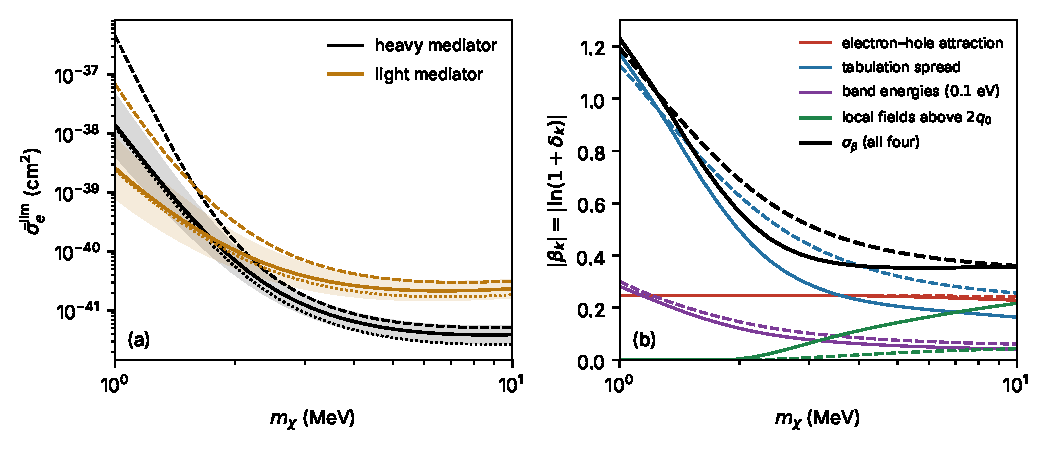
\includegraphics[width=\linewidth]{figures/ch21/fig21_4.pdf}
  \caption{A silicon electron-recoil limit with its theory band. Search: \SI{1}{kg.yr}, every event with at least one pair ($\omega \ge \SI{1.17}{eV}$), no event observed, no background, classical \SI{90}{\percent} limit $N_{90} = 2.303$; standard halo, $\rho_\chi = \SI{0.3}{GeV.cm^{-3}}$. (a) Nominal limit (solid) from the random-phase loss function with local fields of the Knapen--Kozaczuk--Lin tables, whose scissor sets the bands at the measured gap at zero temperature, the band \cref{eq:21.4-band} of the nominal limit (shaded), the profiled limit (dashed; Neyman construction with the nuisance parameter at its conditional best fit, $\ee^{\sigma_\beta^2N_{90}}$) and the limit at the random-phase level without local fields (dotted), for a heavy (black) and a light mediator (ochre). (b) Sensitivities $|\beta_k|$ of the four uncertainties of \cref{we:10-band3}, heavy (solid) and light mediator (dashed). The attraction template is $\delta_{\mathcal{X}} = +0.28$ for $\omega \le \SI{10.5}{eV}$ and zero above, which overstates it above \SI{3}{MeV}, where the compensating weight of the $f$-sum rule enters the window. The other three are the tabulation spread (ratio of the independent-particle rates of the Essig et al.\ and Knapen--Kozaczuk--Lin tables), band energies shifted by \SI{0.1}{eV}, and the random-phase value in place of local fields above $2q_0 = \SI{7.46}{keV}$. Black: their quadrature sum $\sigma_\beta$. Below \SI{1}{MeV} the first energy bins of one table make the spread unreliable. Above \SI{10}{MeV} the momentum range of the other, \SI{22.5}{keV}, truncates the heavy-mediator rate.}
  \label{fig:21-band}
\end{figure}

\begin{workedexample}{The band of a silicon limit from the random-phase level}\label{we:21-rpaband}
Take $\mchi = \SI{3}{MeV}$, a heavy mediator, \SI{1}{kg.yr} of silicon, a one-pair threshold, no event and no background, so that $N^{\mathrm{up}} = N_{90} = 2.303$ and $\sigmae^{\mathrm{lim}} = N_{90}\times\SI{e-37}{cm^2}/\mathcal{R}$, with $\mathcal{R}$ the rate per kilogram-year at $\sigmae = \SI{e-37}{cm^2}$ (\cref{eq:1.5-limit}). The tables place the conduction bands at the measured gap of \SI{1.17}{eV} at zero temperature, and the rate is counted from it (\cref{sec:10.10}).

\emph{The random-phase level.} With the random-phase loss function of the tables, $\mathcal{R} = \num{2.494e4}$ and $\sigmae^{\mathrm{lim}} = \SI{9.23e-42}{cm^2}$.

\emph{The computed step.} The local fields have been computed, and they move the central value, not the band. They lower the rate to \num{1.855e4}, a factor 1.345, and the nominal limit is $\SI{1.24e-41}{cm^2}$.

\emph{The band.} The four uncertainties of \cref{we:10-band3} have, by \cref{eq:21.4-beta} with one bin, $\beta_{\mathcal{X}} = -0.247$ (attraction), $-0.289$ (tabulation spread), $+0.078$ (band energies) and $-0.064$ (local fields above $2q_0$). Their quadrature sum is $\sigma_\beta = 0.393$, and \cref{eq:21.4-band} gives
\begin{equation*}
  \SI{8.38e-42}{cm^2} \le \sigmae^{\mathrm{lim}}(\vartheta) \le \SI{1.84e-41}{cm^2} .
\end{equation*}
The attraction and the tabulation spread carry \SI{93}{\percent} of $\sigma_\beta^2$. Taken one at a time to $\vartheta_k = \pm1$, the four move the limit by factors of 1.28, 1.34, 1.08 and 1.07. The random-phase limit lies in the lower part of the band, at 0.74 of the nominal value against the lower edge at 0.675.

\emph{The profiled limit.} With no events \cref{eq:21.4-profile} is exact, the factor is $\ee^{\sigma_\beta^2N_{90}} = 1.427$, and $\sigmae^{\mathrm{lim,p}} = \SI{1.77e-41}{cm^2}$.

\emph{The detector.} Suppose the efficiency is calibrated to \SI{10}{\percent}, a normalization with $\beta = -\ln 1.10 = -0.095$. Then $\sigma_\beta = 0.404$, the band widens from a factor 1.481 to 1.498, and the profiled factor grows from 1.427 to 1.457. At this calibration the detector adds about one percent to the band and two percent to the profiled limit.
\end{workedexample}

\subsection{One-sided nuisance parameters and excluded cells}\label{sec:21.4-onesided}

A template whose sign is known calls for a constraint that respects it, $\vartheta_k \ge 0$ with the weight $\ee^{-\vartheta_k^2/2}$ on that side, a half-normal constraint. The cost of a half-normal constraint depends on the direction in which the template moves the signal. If $\vartheta_k > 0$ raises the signal, so that $\beta_k < 0$, the statistic at fixed nuisance parameters, \cref{eq:D.47-tfix}, increases with $\vartheta_k$ at every cross-section, and so does the constraint term. The profile then sets $\vartheta_k = 0$ at every cross-section, the parameter costs nothing, and the limit at $\vartheta_k = 0$ is the conservative end of its band. The attraction of \cref{we:21-rpaband} is of this kind: it raises the rate near the gap in every calculation of \cref{sec:10.5}. Only the three other nuisance parameters, with $\sigma_\beta = 0.306$, are then profiled: the profiled factor falls from 1.427 to 1.240 and $\sigmae^{\mathrm{lim,p}} = \SI{1.54e-41}{cm^2}$. The attraction can only strengthen the limit, by 1.28 at $\vartheta_{\mathcal{X}} = 1$. If $\vartheta_k > 0$ lowers the signal, the unconstrained minimum of the profile already lies at $\vartheta_k > 0$, since data without an excess prefer less signal, and the one-sided constraint costs as much as a two-sided one. Linear spin-wave theory, for example, overstates the one-magnon weight of NiO by an estimated $\Delta S/|\vect{S}| = \SI{7.8}{\percent}$ (\cref{sec:14.1}), and that template, of known sign, lowers the signal. Both statements need the template to have one sign in every bin and the bins to be free of excess, so that every weight $a_j$ is positive.

Some cells of the $(\vect{q},\omega)$ plane have no controlled central value, and a limit can be set without them. Removing nonnegative signal from bins without an excess lowers the statistic at every cross-section, so the limit can only rise (\cref{app:D.47}); for one bin it rises by $1/(1 - f)$, with $f$ the removed share. Near the pair-breaking edge of aluminum the conserving loss function changes with the mean free path by more than \SI{10}{\percent} below $y = \omega/\Delta_{\mathrm{BCS}} = 3$, and those energies are excluded (\cref{sec:15.2-nuisance}). At \SI{1}{keV} with a light mediator they hold \SI{20}{\percent} of the rate for the bulk gap and \SI{37}{\percent} for the film gap (\cref{we:15-alrate}), and excluding them weakens the limit by 1.25 and 1.59. For a crystal with a mean free path of at least \SI{10}{\micro m} the clean loss function holds there, and the cells can be restored. The silicon Migdal rate has a region of this kind as well: the coherent zero-phonon response between \SI{0.75}{keV} and $2q_{\mathrm{BZ}}$ is not sized (\cref{tab:12-nuisances}). It carries \SI{33}{\percent} of the rate at \SI{2}{MeV} and \SI{7}{\percent} at \SI{3}{MeV}, so excluding it costs factors of 1.49 and 1.08, and below \SI{1}{MeV}, where it carries nearly all of the rate, no Migdal limit survives the exclusion. In a bin with an excess the argument fails, and removing signal there can strengthen a limit; such a bin needs the full likelihood.

\subsection{The dominant uncertainty of each channel}\label{sec:21.4-dominant}

\Cref{tab:21-dominant} reads the uncertainty budgets of the chapters along the other axis and gives, for each channel at a reference point, the rows that dominate its band. The dominant rows are missing calculations or missing data. The silicon electron recoil lacks a finite-momentum Bethe--Salpeter calculation and a converged independent-particle table, the phonon-assisted window its finite-$q$ form factor and pair-channel screening, the Migdal rate its coherent region and off-diagonal local fields, and NiO its anisotropy. The data that are missing are the cold absorption edge of silicon, the background tensor of ZrTe$_5$ and the gap of an aluminum film. Near the edge of every channel the threshold rows dominate: a gap shift of \SI{10}{meV} weakens a silicon limit \SI{0.005}{MeV} above the edge by a factor of 231 (\cref{we:21-gapshift}).
\begin{table}[tbp]
  \caption{Dominant theory uncertainties of the limit in each channel, read from the uncertainty budgets of the channel chapters. Sizes are factors or shifts of the rate, and hence, for one bin, of the limit. Basis as in those tables: ``computed'', ``model'', ``est.''\ (parametric estimate), ``spread'' (published calculations at the same order), ``data'' (spread of measured inputs), ``bound'' (only an inequality is known), ``unsized''. The last column gives the section, table or figure where the rows are treated.}
  \label{tab:21-dominant}
  \centering\scriptsize\setlength{\tabcolsep}{3pt}
  \begin{tabular}{@{}>{\raggedright\arraybackslash}p{0.20\linewidth}>{\raggedright\arraybackslash}p{0.14\linewidth}>{\raggedright\arraybackslash}p{0.40\linewidth}>{\raggedright\arraybackslash}p{0.09\linewidth}>{\raggedright\arraybackslash}p{0.10\linewidth}@{}}
    \toprule
    Channel & Reference point & Dominant uncertainties & Basis & Section \\
    \midrule
    Electron recoil, Si, density coupling & 1--\SI{3.6}{MeV}, heavy mediator; up to \SI{10}{MeV}, light & tabulation spread: $\times3.2$ at \SI{1}{MeV}, $\times1.34$ at \SI{3}{MeV} (heavy), $\times1.29$ at \SI{10}{MeV} (light); band energies \SI{0.1}{eV}: $\times0.75$ at \SI{1}{MeV} & spread & \cref{sec:10.10}; \SI{1}{MeV}: \cref{fig:21-band} \\
    Electron recoil, Si, density coupling & 3.6--\SI{10}{MeV}, heavy mediator & electron--hole attraction $\times1.28$, $\times1.26$ at \SI{10}{MeV} (known sign); local fields above $2q_0$ $\times1.24$ at \SI{10}{MeV} & model; spread & \cref{sec:10.10} \\
    Electron recoil, velocity couplings & \SI{10}{MeV} & density--current cross term: rate at least 16 (independent particles), about 29 (screened) times the static-electron formula & bound & \cref{sec:10.4} \\
    Core electrons, Ge $3d$ & about \SI{30}{MeV} & crystal final states: $3d$/valence 0.07 against 0.69 & bound & \cref{sec:10.6} \\
    Phonon-assisted electron recoil, Si & 0.333--\SI{0.43}{MeV} & finite-$q$ form factor, factor 3; screening relative to the optical calibration, pair channel not sized; cold absorption data, rate $\times9$ at \SI{0.36}{MeV} & est.; unsized; data & \cref{tab:13-nuisances} \\
    Migdal effect, Si & up to \SI{3}{MeV}; above & coherent zero-phonon response from \SI{0.75}{keV} to $2q_{\mathrm{BZ}}$, \SI{33}{\percent} of the rate at \SI{2}{MeV}; off-diagonal local fields, $\times1.2$ to 1.4, lower end not bounded & unsized; model & \cref{tab:12-nuisances} \\
    Nuclear recoil, Si, multiphonon & \SI{30}{MeV}, $\omega_{\mathrm{th}} = \SI{100}{meV}$ & computed phonon frequencies against measured, \SI{0.24}{\percent}; free recoil in place of the crystal response (evaluation error) $-\SI{6.8}{\percent}$ & computed & \cref{sec:11.9} \\
    Polar phonons, GaAs & single phonon & $Z^*/\varepsilon_\infty$: \SI{2}{\percent} from the measured splitting; a semilocal $\varepsilon_\infty$ moves the rate by \SI{37}{\percent} & data; computed & \cref{sec:11.9} \\
    Magnons, NiO & near \SI{3}{MeV}; lightest masses & one-magnon weight high by \SI{7.8}{\percent} (known sign) against the two-magnon continuum, $+\SI{7.3}{\percent}$ at other energies; magnetic anisotropy near the lightest masses & est.; model & \cref{tab:14-nuisances} \\
    Superconductor, Al & \SI{1}{keV}, light mediator & gap of the sensor, bulk against film: $\times1.23$; edge remainder $-2$ to $+\SI{9}{\percent}$; $y < 3$ excluded, $\times1.25$ (bulk) or $\times1.59$ (film) on the limit & data; computed & \cref{tab:15-nuisances} \\
    Dirac material, ZrTe$_5$ & 20--\SI{1000}{keV}, light mediator & background dielectric tensor: reach band $\times2.8$ & data & \cref{we:16-band} \\
    \bottomrule
  \end{tabular}
\end{table}

For the silicon electron recoil at \SI{3}{MeV} two calculations would remove \SI{93}{\percent} of the variance: a finite-momentum Bethe--Salpeter calculation and an independent-particle table that passes the $f$-sum test at small $q$ (\cref{sec:10.10-open}). With the band energies and the local fields above $2q_0$ left, the band of \cref{we:21-rpaband} would shrink from a factor of 1.48 to 1.11.
